\subsubsection{System Linux, nagrywanie na pendriva}
\begin{wrapfigure}[6]{r}{0.5\textwidth}
                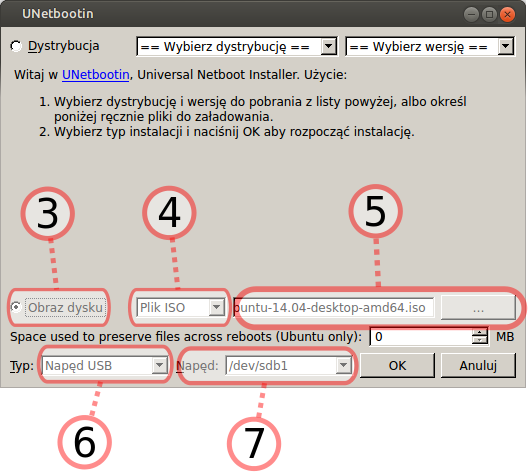
\includegraphics[width=\linewidth]{images/instalacja_nagrywanie_obrazu_linux.png}
\end{wrapfigure}

W systemach operacyjnych Linux do nagrywania obrazu na pendrive'a najlepiej posłużyć się programem \textcolor{ubuntu_orange}{UNetbootin}, dostępnym w każdej dystrybucji. Podłącz do komputera klucz USB, z którego chcesz potem instalować Ubuntu.
\begin{enumerate}[label=\protect\circled{\arabic*}]
\item Zainstaluj UNetBootIn korzystając ze swojego menadżera pakietów.
\item Uruchom zainstalowany przed momentem program.
\item Zaznacz pole Obraz dysku
\item Z menu wybierz Plik ISO
\item W tym polu podaj ścieżkę do pobranego wcześniej obrazu instalatora Ubuntu. Wciśnij przycisk oznaczony trzema kropkami (“\ldots”) i wskaż plik.
\item W tym menu wybierz Napęd USB
\item Z tego menu wybierz podłączonego wcześniej pendriva.\\
\textbf{UWAGA: Wszystkie dane znajdujące się na tym nośniku zostaną skasowane!}
\item Kliknij przycisk OK aby rozpocząć nagrywanie
\end{enumerate}
\subsubsection{System Linux, nagrywanie na DVD}
%TODO potrzebny obrazek z włożoną płytą DVD i wybranym obrazem ubuntu 14.04
\begin{wrapfigure}{l}{0.5\textwidth}
                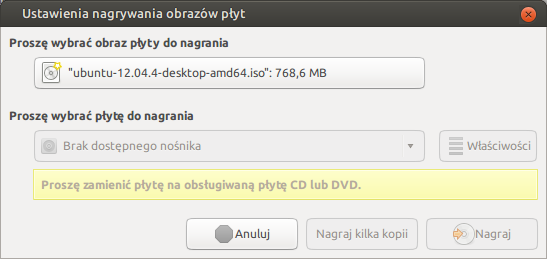
\includegraphics[width=\linewidth]{images/instalacja_nagrywanie_obrazu_linux_DVD.png}
\end{wrapfigure}

Aby nagrać obraz na płytę DVD potrzebujesz odpowiedniego programu. W tym przykładzie posłużymy się dostępną w większości dystrybucji nagrywarką Brasero. Kliknij prawym przyciskiem myszy na pobrany wcześniej obraz instalatora Ubuntu, wybierz \textcolor{ubuntu_orange}{Otwórz w\ldots}, a następnie wybierz \textcolor{ubuntu_orange}{Brasero}. W otwartym oknie zostaniesz poproszony o włożenie czystej płyty DVD. Zrób to, a następnie kliknij na przycisk \textcolor{ubuntu_orange}{Nagraj}.
\clearpage
